\chapter[SCP-001 破碎之神]{
	SCP-001 TwistedGears/Kaktus -The Broken God \\
	SCP-001 破碎之神
}

\label{chap:SCP-001.the.broken.god}

\begin{figure}[H]
	\centering
	\fbox{
\includegraphics[width=\linewidth]{images/SCP.001.the.broken.god.png}}
\end{figure}

\cl{

\GG{\bb{根据O5议会指令}}

\Gg{\bb{下列文档描述了Maksur级异常实体}}

信息受5级机密保护。Maksur级信息的泄露被严厉禁止,且将对SCP基金会及其利益造成严重威胁。访问文件的人员须提供5级安保许可,并接受了对AZ109模因危害的预防接种。未能遵照者将在访问文件时立即遭致“携带者奥米茄”模因处决。

\tred{[提交5级安保许可]}

\tred{[安保认知危害启动]}

}

\begin{figure}[H]
	\centering
	\{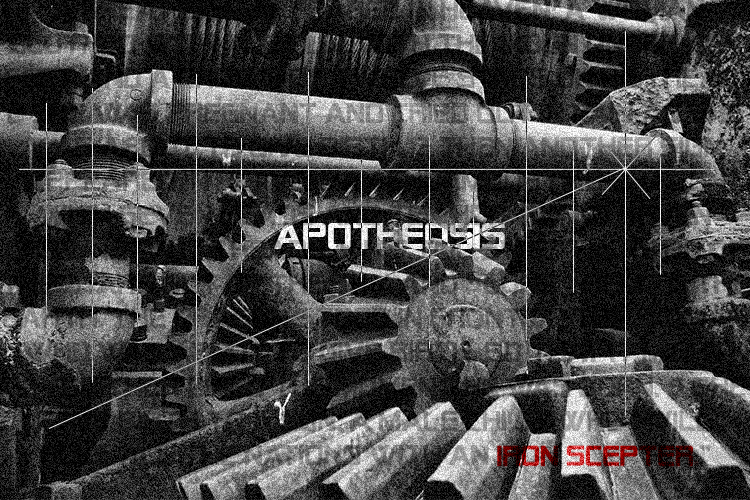
\includegraphics[width=\linewidth]{images/SCP.001.the.broken.god.2.jpg}
\end{figure}

\cl{

\bb{侦测到生命迹象}

\bb{模因接种查明}

\bb{欢迎,监督者}

}

\hr

\begin{figure}[H]
	\centering
	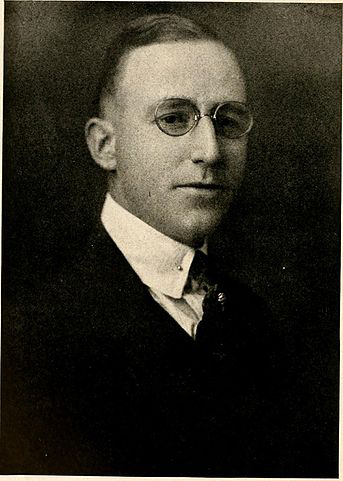
\includegraphics[width=0.5\linewidth]{images/SCP.001.the.broken.god.3.jpg}
	\caption*{Robert Bumaro,破碎之神教会现任领导者。日期未知。}
\end{figure}

\bb{项目编号:}SCP-001

\bb{项目等级:}Maksur\footnote{Maksur分级在1981年由基金会收容委员会联合监督者议会、站点主管议会、基金会伦理委员会联合编入规范。在Maksur级被规范化前,SCP-001曾被编为“Neutralized”,Maksur分级被制定用于替代此不当分级(参加机密委员会记录CA-10931“Neutralized分级在分标准应用中的关联性” CA-10945, “提案:Maksur级”)}

\bb{特殊收容措施:}相关异常项目与SCP-001间存在关联性的信息将在各自文件中被删改。这些项目与破碎之神教会的关联可以保留,但其来源将被删改或模糊处理。

SCP-001的非活跃部件将被留在原地,在其所处区域内禁止任何行船或潜水。平民对SCP-001的察觉将被压制,并使用记忆删除以维持保密。破碎之神教会相关人员若做出寻找SCP-001非活跃部分的举动,将被基金会拘留并审问。关于SCP-001的一切信息,无论是实体还是数据,都将被没收收容。

SCP-001的非活跃部件被预期将保持在无活动状态;然而,若SCP-001出现自发复苏,所有在Site-27, Site-44, Site-90及Site-101附近的活动中机动特遣队单位将被派去采取收容措施。若该事件(当前编为001-登神事件)在现代世界发生,确信当前采取的信息压制措施不足以应对之。001-登神事件极有可能导致一次SK级“破碎面纱”情景\footnote{SK级情景将自动使基金会全部敏感信息备份到自我收容的“深井”站点(当前117、118和119)内最高级安保服务器中。所有非必要人员将接受人工记忆删除治疗,所有主要地方站点将进入全面封锁。当前模型下,该状态尚不确定。},之后将可能是XK级“世界末日”情景。

现存仍活跃的SCP-001部件任何情形下不得进入非活跃部件周围20km内。

\bb{描述:}SCP-001是一系列异常物体之集合,此前曾是破碎之神教会在1942年晚期于墨西哥拉巴斯组装的单一巨型机械实体。这些物体包括\hyperref[chap:SCP-217]{SCP-217},\hyperref[chap:SCP-1139]{SCP-1139},\hyperref[chap:SCP-882]{SCP-882}和\hyperref[chap:SCP-629]{SCP-629}的部分内部零件\footnote{在与破碎教会线人合作收容\hyperref[chap:SCP-629]{SCP-629}后才发现此事。未知这些部件是如何被 Wondertainment博士在基金会及破碎之神教会内部线人不知情的情况下收集到,也不知\hyperref[chap:SCP-629]{SCP-629}自身是否知晓自己与教会的联系。}。完整列表参见\red{这里}。

教会成员将这些异常物体组装在一起,意图以此修复他们信奉的神明。在启动后,据报告SCP-001开始将金属物体整合到自身之中,并开始积极寻找其他异常物体。SCP-001,以及因其被组装而引发的“001-登神”事件,造成了西墨西哥环境发生剧变,并引起了有记载以来最大范围的一次记忆删除施用。在事件后,仍然活跃的SCP-001部件被基金会带回站点收容,非活跃部分则被留在了加利福利亚湾底部,约在23.807269,-108.418369处。

\bb{附录001.01:}描述SCP-001的已收集信息

\begin{scpbox}

\ii{Jorge Castillo神父的陈述抄录,1945年8月}

Fernand是第一个…我觉得,是他们找到心脏后第一个联系我的。他们描述它的方式,还有眼中的狂热,令我迷惑,接着我知道了。我知道他们已经完成了。

在我姐姐的坚信礼后我在周末与Anthony及Salvador见了面…当他们向我展示时我被惊住了。它简直就是一堆齿轮、活塞、发条零件和上油金属部件的混合体,每个部件忠实地相互搅动且没有动力来源。在内部我看到了心脏,一如他们所描述。

它对我说话了。不像你与我这种对话,而是…用图像和感觉。还有痛苦。它处在如此的痛苦中。就像那曾经赋予它生命的火花也让它察觉了自己为何物,又或者不是何物,它只愿再次完整。

愿望这个词也许太过了。不是愿望,更多的是冲动。那造物中的什么东西驱使它向着不假思索、不会动摇的结局前进。他们呈现给我的这个造物和我曾发现并祝福的一切器物都不同。这一个不一样,它有什么地方不对,直到他们完成我才明白过来…

我请求Salvador把它带回\hyperref[chap:SCP-2217]{海岸}拆除,这样是不对的,但他们不可能听进去。在我离开前它已经开始动了。从一头到另一头开始振动,开始走动了。它蹒跚着走过一个扳手,那扳手就变成了它的一部分。他们对我说,“我们的神不破新生了!”

我再没见过他们。

\end{scpbox}

\begin{scpbox}

\ii{1946年对Francis Bollinger的采访}

它不用语词,或者任何语言。它发出金属的声音但同时…当我们靠近图像和概念就涌入了我们心中。你可曾感觉到,当你有了一个思绪或念头-它完全就在那,在你的思维中完整地诞生-但你还是必须去思考与之对应的语言,虽然你在完成句子前就知道了观点?那就像是这样,但却是来自另一个心灵。真正的神之言。

\end{scpbox}

\begin{scpbox}

\ii{2007年对特异事故调查单位特工Trixie Silva的采访}

那里有几个狼-等等,你们知道那是啥对吧?他们就像…就像猎人,为地平线倡议工作。他们在圣玛格丽塔的教堂附近遇到了我们,要我们交出从破碎之神教会那里招来的东西,就像以前我们移交过的亚伯拉罕类物品。

我们讨论起应不应该交出去-我们和地平线的立场有些动摇,更多是最近的事情。我们和当地的破碎教会关系不错,但这些狼…好吧要更有攻击性。我们看着手里的东西,这时候那个女人走了过来。我不知道她从哪里来的。她穿的就像嬉皮士;很瘦,头发上绕着铁链,但她看起来和整个时代完全不合。她眼睛里的凝视,她诡异的笑容,就像她几乎不在那里。

她看着我们拿的东西说她就要这个,噢。我其实并不清楚那到底是什么。一个金属盒子,呼呼又咔嗒地响着,我捡起来的时候边缘还放出了点光。比我原以为的还要亮些。我问这对她为什么那么重要,她说向我展示要比说简单。

她闭上眼低下头。之后她没有动也没有说,我也只好把眼睛闭上了。她把额头靠向我的,但有点分开。我们站了大概一秒,foi muito estranho,接着她突然把下巴往下挪了挪,让我也被向下一拉。

世界在我脚下掉落,我坠了下去。有什么东西在我的思绪里咔哒作响,是一幅双齿轮的图像,先是紧密结合,现在分离开来。我感到脊柱的骨突随我弯腰而伸展,只一步我便同行星这多维的螺丝钉合在一起。它环绕太阳熔炉旋转,被重力锁链所牵引,我们用弹簧无限拉伸的力量,一并飞过这多油的宇宙…

…抱-抱歉。这是一次体验。不,不是宗教体验。但…对。她让我把盒子捡起来,我感觉它好像重了点。我分不清到底是真变重了,还是我感觉它更加…重要了。我把盒子交给她,完全没听到狼或者队友或者上级的声音。

\end{scpbox}

\bb{附录001.02:}1945年6月对被开除的前破碎之神教会牧师Dolorous Randall神父的采访。

\begin{figure}[H]
	\centering
	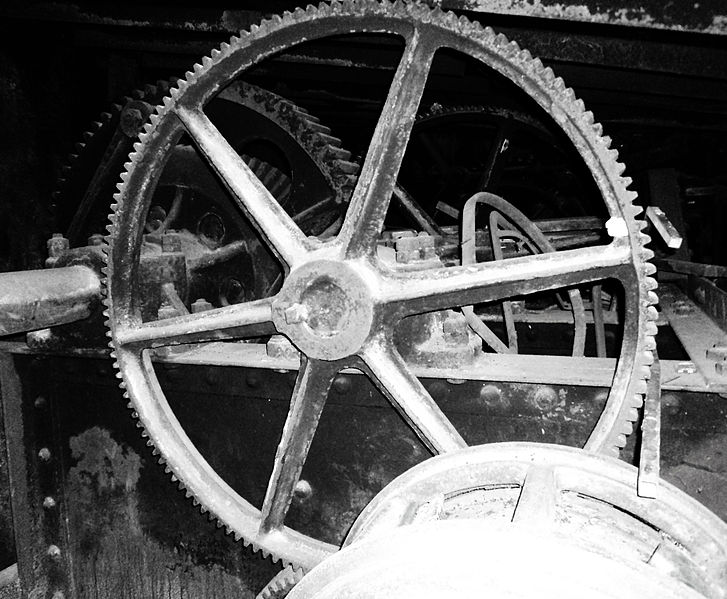
\includegraphics[width=0.5\linewidth]{images/SCP.001.the.broken.god.4.jpg}
	\caption*{在破碎之神教会仓库拍摄的照片。被确信为SCP-001的早期化身。}
\end{figure}


\begin{scpbox}

[多余部分略去]

\bb{Williams:}好了。你早先提到了心脏。他们找到它的时候你可在场?

\bb{Randall:}不,完全没有。那时我在国外,在巴拿马处理一个新任务。我只在事后听说了Ezekiel。

\bb{Williams:}Ezekiel是谁?

\bb{Randall:}Bumaro的一个特工。他身边总有这么一群人,与神协调能感受它的存在,与它对话。Ezekiel曾经发现了个挺重要的器物,Bumaro随后让他加入了。这些特工也是第一批接受改造实验的。如你所想,死了很多。

\bb{Williams:}但Ezekiel没有?

\bb{Randall:}没有。他和Bumaro很亲近,我不知道他会不会拿Ezekiel的健康冒险。这不重要,Ezekiel不需要改造也能与神对话。他就是…能够。

\bb{Williams:}所以Ezekiel对心脏做了什么?

\bb{Randall:}你听Avery说过他们有一大堆器物储备,对吧?这些特工碰过的任何东西,只要他们在其中感觉到了什么,就会被送到拉巴斯和其他的放在一起。大部分都是无价值的,但迟早他们会发现正品。精炼者,那一个-无论你们怎么称呼,一个特工在尼泊尔附近发现了它。他们有了筋腱和韧带等等一切,但都是只是部件。它们都可以自己活动,但不能在一起做什么。

\bb{Williams:}你什么意思?

\bb{Randall:}经典说神会在碎片被带到心脏面前时自行重整。只需要把手臂交给心脏,神就能得到一根手臂。但他们就是找不到心脏。他们(停顿)几个特工曾宣称找到了,但仍是和其他部分一样的无用机械碎片。

\bb{Williams:}Ezekiel在这之中是什么角色?

\bb{Randall:}Ezekiel 是那个告诉Bumaro,如果找不到心脏也许可以自己做一个的人。很快就知道这计划不会持续到夏季过完。我在Ezekiel走后被派去为他们找补给,他们的供应快要耗尽了。

\bb{Williams:}我们的记录显示心脏是被发现的。这不是真的?

\bb{Randall:}当然不是真的。你肯定不能给教众宣道说神把他的部件赐予你然后转身又说其实大部分基础部件都是你自己凭空拼造的。但至少比没有好。他们创造心脏并让它活过来的细节从没向我透露,但我能从蛛丝马迹里得到结论。那年有过一次旱灾,脊髓灰质炎危机又史无前例严重。数千人死亡,都是自然原因。一次可怕的事件,因为注意力都在战争而从未被准确记录过。神啊,但谁说得清呢。

\bb{Williams:}你觉得这两者有联系?

\bb{Randall:}我觉得时机太巧了。而且既然我知道那东西最后变成了什么,我想答案很清楚了。那不是神之心脏,特工。那是完全不同的什么东西。

[多余部分略去]

\end{scpbox}

\bb{附录001.03:}回收到的视频抄录,1942年11月

\begin{scpbox}

\ii{视频回收紫当地纪录电影团体。}

镜头从被破坏的房屋开始,车库周围满是残骸。金属碎片和橡胶条痕迹从车道延伸到沥青路,之后继续到街道上。各种车辆残片散落在街道和沿街上。这些痕迹引向正在将一辆卡车吞入自身底盘的SCP-001。

SCP-001继续向最近的房屋前进,开始吞食排水沟。区域居民逃离现场,多人被SCP-001丢下的玻璃渣和扭曲金属击伤。SCP-001身体的多个部分发出光芒,照在多个跪伏的人影上。SCP-001继续沿街道搜寻更多材料源,其底盘上一个部分变形从主体上落下。

伸出的部分继续变形,形成一个类似人类脊柱及肋骨架的垂直荚体。荚体多处破损,肋骨状突起从中伸出,其余荚体变形为一高约3米的人形实体。光从其头部发出,投在附近的平民上。

金属人形抓起似乎已死亡的平民,将其放入肋骨间的小空间内。肋骨随人形实体靠近第二名试图爬走的女性平民而摆动。实体将挣扎的平民举起放入胸腔内。之后人形实体转身背对摄像头向第三人前进,似乎是女子断手的物体掉落在地。

人形实体的后背上随其收集人体而长出一缓慢增大的赘生物,人形实体的身体大小也随之变小。在吞噬到第六人后赘生物已经大过了人形,使其无法再两足行走。其肢体已收回体内,肋骨伸出使其爬上了附近一栋房屋的屋顶。

它在原地停留了20分钟。球状物外层破裂后从内部裂开,露出三个人形实体。它们看起来是SCP-217感染者,表现出六名被吞食平民的身体特征。其中一名女性头皮上连着锁链,摇晃着另一个似乎已死亡的个体。第三人是一长着发条胳膊的男性,检查自己后跳下了楼顶,腹部着地。它似乎并未因此受伤,令其更为紧张。之后它开始追赶在街道远处吞噬其他汽车的SCP-001。

女性人形注意到了摄像者,开始挥手,但很快停止。它看向SCP-001后跳入后院,离开镜头中。

\end{scpbox}

\bb{附录001.04:}与Robert Bumaro谈话的电话录音。 \\
\ii{备注:下面破碎之神教会一名特工(姓名未知)和Robert Bumaro的电话交谈录音。该次通话记录在1942年12月,由基金会人员在1966年对一处教会据点进行搜查时获得。}

[播放音频]\footnote{
编者\QIS:在\href{http://scp-wiki-cn.wikidot.com/twistedgears-kaktus-proposal}{文章的Wiki页面}上此处是一个Flash控件,点击按钮可播放音频。由于大多数PDF不支持交互操作,所以没有导入。可以点击\href{http://scp-wiki.wdfiles.com/local--files/twistedgears-kaktus-proposal/bumaro.mp3}{这里}访问该音频。
}

\begin{scpbox}

[通话开始]

\bb{Bumaro:}你好?

\bb{Agent:}祝福您圣父。

\bb{Bumaro:}Dmitri?

\bb{Agent:}不。

\bb{Bumaro:}哦,当然。祝福你,孩子。小主如何了?

\bb{Agent:}日渐强壮。我们已将他从办公室后面挪入了附近的仓库。

\bb{Bumaro:}喂过他了吗?

\bb{Agent:}如您要求。

\bb{Bumaro:}很好。你何时去Puerto Peñasco?

\bb{Agent:}本周内。我们就等下列车。

\bb{Bumaro:}可能还得快点。几周前拉巴斯被突袭了一次。我们有三个人没有被找到。基金会活动越发活跃在-(暂时挂断)

\bb{Agent:}圣父?

\bb{Bumaro:}(对背景的某人)明天,明天。

\bb{Agent:}圣父?

\bb{Bumaro:}是的。我们曾期望他们北上,但他们却去了西边。小挫折。

\bb{Agent:}那安全屋呢?有将近一百件其他器物在那里,而且—

\bb{Bumaro:}(打断)小挫折。他们不知道在哪,就算他们知道了,这也不是他们的优先项目。他们的眼线,还有他们在世界上的其他眼线,都注视着欧洲。只要他们的目光落在那里,就不会发觉我们的完成直到已经无力阻挡他。

\bb{Agent:}这,嗯,还有其他事想问您,圣父。

\bb{Bumaro:}是的?

\bb{Agent:}我们的神,呃…太饿了。我们似乎无法满足他,我们得到的供给不—

\bb{Bumaro:}(再次打断)问题是什么?

\bb{Agent:}圣父,我们的…主在吃他自己的住所。我们无法劝服他停下,不能和他讲理,它-

\bb{Bumaro:}胡说。虔诚的心可以与神直接对话。当他靠近时你不能听到他的话吗?没有感觉机械在你心中运转?或者连在眼前呼吸鲜活的神也不能让你坚信?

\bb{Agent:}不!圣父,不是这样,是-

\bb{Bumaro:}我不会再听了。这么多年,我们祈祷、期盼神在我们面前不破新生。现在,他已展现了自己。我们知道神会对虔诚之心开口。如果你要告诉我,你们中连虔诚到能与神沟通的人都没有,现在就告诉我把你们换掉。

\bb{Agent:}我们的信念依然坚定,圣父。请您原谅我的无礼。我只是迷途了。

\bb{Bumaro:}那就自己反省。我担心你的信念。去找个弟兄,找个信念比你坚定的,让他去和主对话,告诉他保密的必要。我们的主将会理解,毫无疑问。不破之神是一位理智的神。

\bb{Agent:}是的,祝福您圣父。

\bb{Bumaro:}祝福你,孩子。

[通话结束]

\end{scpbox}

\bb{附录001.05:}增补报告,1943年12月 \\
\ii{下面是对基金会Site-74指挥官Mark Peterson的采访。主管在001-登神事件前驻扎于墨西哥城,事件期间与拉巴斯的基金会人员一同在站。}

\begin{figure}[H]
	\centering
	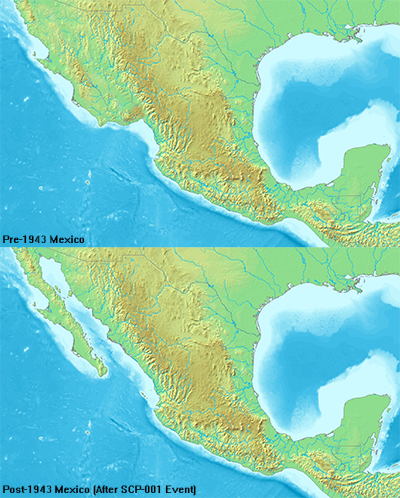
\includegraphics[width=0.5\linewidth]{images/SCP.001.the.broken.god.5.png}
	\caption*{001-登神事件前后的墨西哥}
\end{figure}

\begin{scpbox}

\bb{Director Cornwell:}从头再来一遍,我们在记录。

\bb{Commander Peterson:}好。关于教会活动的第一次报告是在41年,但那时候还都是非常小的事。我们刚刚完成了北部边境附近的外勤行动,正要准备把资产搬去亚特兰大准备法国的任务。我们已经接到命令,去收回一些他们不愿意被德国佬抢去的敏感物品。他们还准备派出我们整个部门去完成此事。领导不确定罗斯福会不会打电话为我们留下充足时间协同美军,所以我们必须得单独前进。

\bb{Director Cornwell:}你为何留在拉巴斯?

\bb{Commander Peterson:}我完全是偶然在那。我们的一辆列车取道往拉巴斯的陆路,也许是要顺路去取回一些军备。结果那趟列车本来是要北上的。所以突然之间大部分格兰德河以南的领导层就跑到了拉巴斯来,回想起来从整体效果看这倒可能帮了我们大忙。

\bb{Director Cornwell:}你何时首次听闻001-登神实体?

\bb{Commander Peterson:}(笑)耶稣啊。现在他们这么叫那东西了?那个机器,我猜, 我们第一次听说,是有本地活动频繁的风声,在…我猜大概得是一年多以前。我们在42年10月到了拉巴斯,所以…对,听起来没错。我们搞的第一个确凿证据是在一辆… 难民车?虽然这么叫着很傻但我想是准确的。他们在十月末来到拉巴斯,说整个镇子都被盖住了。他们没有真正的解释什么,就是一直说"la máquina, la máquina", 你知道的,“机器”。顺便这就是我们那么叫它的原因。我们还完全不清楚那应该是个什么

\bb{Director Cornwell:}那你和该实体的第一次接触呢?

\bb{Commander Peterson:}好吧,铁路停止运营了,如果你是这意思的话。我们听当地警方说北边出了事故,列车不会再往边境开了。这对我们来说可是大问题,我们可不能坐着几辆车向东走到山脚小镇为止。它们大多都和单独的铁道线完全挂钩,我们本可以就那么走。但是大东西,那些列车要去拉巴斯拉的东西,不能动。所以我们得等着。之后DeMarco想出个注意,派支小队沿铁路看看堵塞在哪,我们能不能清理掉它。他自己领队。

\bb{Director Cornwell:}特工DeMarco怎样了?

\bb{Commander Peterson:}你他妈知道他出什么事了Bill。

\bb{Director Cornwell:}为记录。

\bb{Commander Peterson:}好吧。我们三天没有收到回信,于是准备把剩下的领导层送去东边免得再等了。但五天后DeMarco的一个部下回到了营地。他精神混乱,说着“吞世怪物”,还有其他所有人都被盖掉了的话。他们是被盖掉了不是吗?我知道那时候它还不是最后那么大,但也不是可以应付的东西。DeMarco…

\bb{Director Cornwell:}你没事吗?

\bb{Commander Peterson:}没事。他试过想杀掉它。但接着他也许明白了我们之后才弄明白的事;我们不可能收容这东西。世界上没有哪个洞大到能装下它,或者有什么盒子是它吃不掉的。但这对他没意义了,其他跟着他去的人都是。那机器不关心这些。

\bb{Director Cornwell:}你什么时候第一次看到了它?

\bb{Commander Peterson:}十二月。在我们蹲守期间,我加入探索队溜过去看个究竟。它已经…我是说,你看过它对边境做了什么。我从来没看过大成这样还能动的东西。就感觉是一座活动部件堆成的山染黑了天空,好像它是在烧那些被它铲进胸口的东西一样。然后它又小了!它… 我不知道。我们都接受有XK-事件准备训练,但这个超出或者说在我们受过的任何训练之外。它就是无敌的。我们知道我们是去送死,那东西要杀了我们,只是个时间问题。

\end{scpbox}

\bb{附录001.06: }收集到的基金会通信 \\
\ii{备注:下面是拉巴斯驻扎基金会人员的书面通信摘录,在001-登神事件后回收于临时站点。姓名已隐去。}

\begin{scpbox}

亲爱的███████,

我甚至不知道这封信能不能送到。列车全停了,但指挥官说还能把信送出去。我希望确实如此,希望你能读到。

这里的天空已经暗了好几周了。每天北边都有烟飘来,呼吸都很困难。这里还是没有室内水管,除了我们公司的另一些人外都不说英语。

我们还是不知道我们在这里干什么。我一直听说要修铁路,但为什么不去北边?不是北边的铁路坏了吗?

\end{scpbox}

\begin{scpbox}

今天有个男人来到镇上,基本上半张脸都被煮过一样。他就像个死人,对谁都不回应。他走到镇中间就倒地了。在医务室醒来后,他变得很激动。说什么山一样大的机器还能和你说话。说那里有人从各自家里跑出来,把自己扔到它身上。说他们被碾碎,像是在草坪修剪机下面跳一样。之后他就死了,没人知道怎么回事。

\end{scpbox}

\begin{scpbox}

山脉在我们面前被撞碎。我们看到一个身影从烟中立起,缓慢笨重但势头恐怖。它不是像野兽一样爬行或是人一样走动,而是靠着几百万齿轮转动推进,就如钢铁的眼镜蛇。它的身体向前伸出,进入烟中,高过我们所能触及。在它的胸口里我看见有火在跳动,就像地狱的熔炉。它来到我们北边的山前,却没有停下或是绕路,而是就这么穿了过来,把山峰全部吞噬。它身处一条长胳膊,将整个村庄抓起塞进口中。我看到人们随家园被抹去一并走向死亡,和其他人一起投身地狱中。接着它叫了,不是齿轮的嘎吱或机械的轰响,而是在我们的心里。我能在心里听到它。它在嚎叫。

\end{scpbox}

\begin{scpbox}

\bb{指令:}中央指挥部,Site-001

\bb{敬礼:}█████████████

临时站点损失。拉巴斯成为废墟。机械实体被收容。大规模地理改变。XK已避免。申请记忆删除支持。

\end{scpbox}

\bb{附录001.07:}采访GOC中尉“归来者” \\
\ii{备注:下面是对全球超自然联盟中尉、代号“归来者”的事后采访摘录。采访记录及全部抄录由基金会特工在1992年的协商情报交换中获得。迄今“归来者”的身份仍然未知。}

\begin{figure}[H]
	\centering
	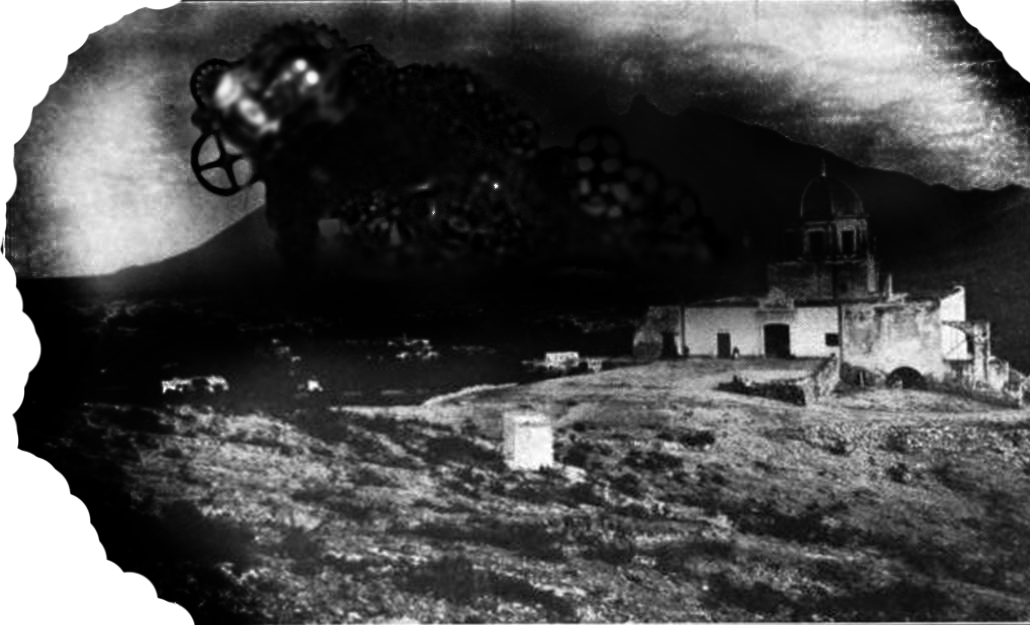
\includegraphics[width=0.5\linewidth]{images/SCP.001.the.broken.god.6.png}
	\caption*{SCP-001,照片拍摄于事件后且严重受损,拍摄者未知}
\end{figure}

\begin{scpbox}

基金会特工里流传着一些故事,就是那种白头老兵在长夜值岗或者在小房间里讲给新兵蛋子的故事。我不知道是谁开的头,但我知道他们现在还在讲。已经半个世纪过去了,他们确实还是对的,你就是可以给他们如此信任。他们说,“你知道么,GOC杀了神。”

但新兵就会说,“不,这不是真的。神被收容在Site-管他是哪呢。反正GOC没有杀过神。”接着他们就会讨论起被他们锁在某处的绿型,那个说自己是基督教上帝的家伙。但这时老兵只会摇摇头,笑而不语。因为他们都知道。

他们都知道在1943年,在末日之中,基金会只能眼看着GOC拯救世界,什么都做不了。

隐喻枪是在希腊海岸边的一座岛上被发现。我甚至不记得它长什么样了,我记得的只剩下记忆删除留给我的那一点模糊回忆。但我本能地觉得它不是你以为的那么重。

为什么记忆删除?那时候我跟着地区部署的分遣队,显然有一块碎片让它造成了心智影响。我模糊地觉得有什么不对,所以我听了他们的话。我不记得它长什么样,我也想不起来它是如何毁掉那么多大陆的。该死,我只记得它何时发生,知道这事的唯一原因还是前后地图的变化。但我还是能感觉到,我的本能说,事情本不该如此。我们站在一个愤怒的复仇神面前,而它做的全部事就是祈求我们杀掉它。

我们全都是如此乐于履职。

\end{scpbox}

\bb{附录001.08:}记录到的视频抄录 \\
SCP-001的较早图像,在附近城镇的撤离中拍摄

\ii{备注:下列是回收的视频录像抄录,长约30秒。抄录在回收后不久被批准,当前视频本身已经损坏无法解读。视频的声音被调节到可接受状态,可在下方播放。\footnote{译注:此处有语音。}}

\bb{回收音频:}警告:声音极大。

[播放音频]
\footnote{
编者\QIS:同前文注。音频文件可点击\href{http://scp-wiki.wdfiles.com/local--files/twistedgears-kaktus-proposal/Apotheosis.mp3}{此处}访问。}

\begin{scpbox}

\bb{00:01:}记录在镇上开始。许多建筑倒塌着火。有明显的剧烈地震活动。

\bb{00:03:}视频移向SCP-001。大小在视频中难以辨认,但该实体占据了整个镜头。它正在缓慢移动。

\bb{00:09:}SCP-001被看到将大块土地移入自身中。偶尔有火焰从实体中迸出。

\bb{00:15:}天空似乎被闪电照亮,可以听到空袭海妖的声音,SCP-001上方的云层突然分开。\hyperref[chap:SCP-2399]{SCP-2399}出现,其下部轻度损坏。可以看到基金会迫击炮从上方飞过。
\bb{00:20:}一发炮弹击中SCP-001。没有造成可见损伤。

\bb{00:22:}SCP-2399的下部开始发蓝。

\bb{00:24:}SCP-2399发出明亮光束击中SCP-001。SCP-001剧烈反应并向 SCP-2399抓去。

\bb{00:26:}巨大爆炸。视频内容不可见。

\bb{00:30:}附近人群尖叫,视频结束。

\end{scpbox}

\bb{附录001.09:}SCP-001的无效化

\begin{figure}[H]
	\centering
	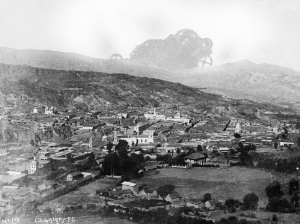
\includegraphics[width=0.5\linewidth]{images/SCP.001.the.broken.god.7.png}
	\caption*{SCP-001的较早图像,在附近城镇的撤离中拍摄}
\end{figure}

于1943年7月17日,全球超自然联盟的特工联系了基金会在墨西哥拉巴斯的主管,请求支援对001-登神实体所在地的运输。基金会特工迅速部署飞机救援GOC人员。抵达后,特工描述称他们获得一个特殊的异常器物,并有可能被用于阻止001-登神实体行动。

在抵达拉巴斯的三天后,于1943年7月24日,全球超自然联盟派出一名特工携带该特殊器物去往001-登神实体所在地。在1943年7月25日早上,在001-登神实体抵达太平洋海岸时另一个巨大的机械构造体\footnote{之后编为SCP-2399并在文件中给予合适掩盖故事。}出现在其上方。该实体的来源未知。

在SCP-2399出现后的事件记录不完整且可能不准确。此次遭遇的结果是SCP-001被消灭。SCP-2399消失,之后以损坏状态出现在木星,当中原因至今未知。

SCP-001剩余的非活跃部分,即一团巨大分散的机械部件,留在了加利福利亚海湾底部。在从非活跃的结构体中取出SCP-882后,剩余部分坍塌彻底停止活动。

在001-登神事件后,对该区域居民进行了代号“下加利福利亚”的大规模记忆删除行动。此次行动因SCP-001周围厚重的黑烟得到支持,当前历史记录将此事件描述为一次森林火灾。大量精力被投入在修正区域地图及搬迁失所平民上。出于对大规模记忆删除规范的需要,多个实验性神经变形器被使用\footnote{特别是U级、UN级和UP级记忆删除,当前都已被终止。},因对其副作用缺乏认知,估计此举造成不少于200万人在001-登神事件后的十年内死亡。

\bb{附录001.10:}收集到的全球超自然联盟文档 \\
\ii{备注:下列文件由POI-004D/001(参见附录001.12)交予基金会人员。当前未知POI-004D/001如何获得此文件。}

\begin{tcolorbox}[colframe=black, boxrule=0.5pt, colback=white, center upper, leftright skip=0.12\linewidth, breakable]

\begin{figure}[H]
	\centering
	
\includegraphics[width=0.6\linewidth]{images/SCP.001.the.broken.god.8.png}
\end{figure}

ATTN:Darius将军

物品回收报告

\bb{编写:}Van Pelt中尉

\bb{C.O:}Baghram上校

\bb{报告长度:}57页

\bb{报告概要:}1942年12月30日,一个具异常性的游荡人形实体在希腊海岸外的小岛附近被巡逻员发现。该实体,宣称没有名字也不能流利用英语交流,携带一个棒球大小的小型立方体器物。实体似乎为女性,其头皮上连着几根钢链。

实体最初愿意交出所带器物(编为AR-213),但很快出现敌意并开始说话。实体对中队人员发出生命威胁,击倒两名人员,随后被Dixon军士制服。实体提及墨西哥西部,要求将其释放把该器物带去那里。

更多调查发现SCP基金会在该区域的活动越发频繁,同时还有一些轻微地理异变。在aghram上校指令下,第二团看守该实体(编为EN-340)开往异变地点。在舰船停靠美国边境后,EN-340开始变得消极,显然不适且心理失常。

建议返回后,在处决前对EN-340进行更多心理评估。一旦对AR-213的分析完成,器物将被送往苏黎世焚毁。

报告附于此以供考察

Lt. R. Van Pelt

第二团

全球超自然联盟维和部队

\end{tcolorbox}

\bb{附录001.11:}Ruberson特工的陈述,1944年1月

\ii{备注:特工Aaron Ruberson在收集SCP-001器物时正驻扎在站。因大部分基金会高级人员被派往参加收集,他被要求进行事后陈述。报告原先存放在 Site-17,之后被加入另一与SCP-001相关的机密材料中。未知是否有其他人员知晓此报告,或者有任何副本被制作。下面是陈述摘录。}

\begin{figure}[H]
	\centering
	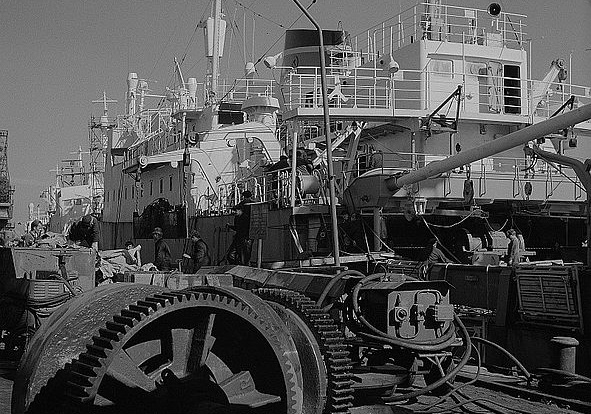
\includegraphics[width=0.5\linewidth]{images/SCP.001.the.broken.god.9.jpg}
	\caption*{SCP-001的非活跃部件正在被装船送往收容。}
\end{figure}

\begin{scpbox}

我们先把能从海岸拿走的拿了。小东西、齿轮滑轮还有活塞,就这一类。大部分都是垃圾,但还在抽动和旋转。它们还是有生命的。这些小零件大概在几小时后死透,但几周后我还是能听到那些大碎片在搅合。就像砍掉鸡头那样。

重要的部分,那些已知是真正教会器物的,被我们打包运往拉巴斯的列车运走。我数了数,基督啊,也许得有一百个?每个都是异常器物。车站有些小伙子笑话说就为存这些东西他们怕是得修个新站点。
 
幸运的是我们把伤亡压得很低。大部分人都只是在机械附近有些懵,就像是不能把手臂拿开一样。Rodriguez的手被压了,我们只好把他送去当地诊所处置。我觉得整个过程里就有一起死亡。一个我们雇来的当地人帮忙潜到海湾下给那个心脏捆上绳子,好让我们把它拉出来。我没看到,但我听说了。说他们发现他的头被碾烂在两个活动部件中间。还说看起来他是自己把自己推进去的。

但我不知道,我没亲眼看见。我倒是有看到标签。

你知道的,当某地制造了什么产品,为了便于辨认其产地,这些家伙总会找个大片金属刻上名字然后在部件一侧给它贴上吧?我们在其他部件上看到了不少这种东西,都是它在一路向海吃过去的途中收集的。不过教会器物都不是这样。它们和其他所有东西一样嗡嗡响,但是没有标志。你站在这些东西前就能感觉到什么,像是安详。整个感觉就像,它感觉很平静。像是解脱。

除了那个心脏。当我们终于把它搬上海湾,因为天气原因我们把它留在岸边放了一天。有些当地人开始发痒。说他们听到声音,不愿意靠近。不管多少钱都不干。只有等到北边的基地派来更多支援才能把它弄上船。

我…伙计我不知道。我见到过各种的这些东西,但我的模因抗性还是很高的。我为这个任务通过了不少测试,一切良好。但我无法抵抗围绕那心脏的另类感觉。我不知道可不可以说听到了什么,但…好吧,标签。我们把它搬上船向北准备离开的时候我第一次看见了。我那时候还没想到要说什么,甚至都没往心里去,知道我看到了其他一些文件。接着船在风暴中沉了,我们丢失了心脏,整个时间我一直在想着那该死的金属标签。接着我想我发现了。那根本不是教会的东西,Johnny。
标签上写的是“工厂所有”\footnote{因近距离检查SCP-882的困难性,这些言论尚未得到证实。}。

\end{scpbox}

\bb{附录001.12:}对POI-004D/001的采访 \\
\ii{备注:下面是2009年对POI-004D/001的采访摘录,此人自称为一此前未知的破碎之神教会分支成员。联系在特异事故调查单位协助下进行,他们曾与POI-004D/001有过互动,详情记录在附录001.01中。}

\begin{scpbox}

所以,给我说说你觉得你们知道的事。

明白了。

有趣。

好吧,你们倒也不是全错。在现在这个时候也是值得称赞的。我感觉你们忽略了几个关键细节,以及高看了某些自认健忘症患者给你们的情报。

那就让我直说好了。

GOC并没有杀死耶和华,虽然他们自傲地如此宣称着。他们消灭的也不是破碎之神。确实,那确实是它的碎片之一,但你会给我个轮轴再把它叫成车么?噢,所以你们把几个部分凑在了一起。也许有引擎了,但仍然不是车。

神比那要更为简单。神是万物。从最大的星到最小的尘。每个小部分,对它们自己都是微不足道的。做着它们应做的事。切合在一起,相互咬合。这全都是宇宙机械的一部分。

这机械的面貌,在某种程度上,就像是一种比喻。一个理念。但我肯定你们也知道,理念是强大的。它们从无中创造出有,或是将已有的加以改变。神的一小束火花闪过,象征成为真实。在一颗生命如此丰盛的星球上,你们产生了无数理念。

你可能要问,“为何要叫它破碎之神?”可能的回答有几个。和翻译问题一样简单的事。被虔信者重新解释得具体了。“破碎”只是对某个更微妙词语的糟糕翻译吗?神是在大爆炸中破碎了吗?如果是这样,它为何破碎?若它被修复又会怎样?

这些问题我一个都无法回答,但你们已经有了答案。到最后,无论神曾经是什么都不重要了。重要的是,对你们而言,它必须保持现状。“破碎”。神知道。那些更强大的部分,传统教派视为圣物的机械部件,它们知道它们本不该成为一个整体。就算迫使其合体,用异己的力量驱动,它们也知道自己本真为何。怪兽的啃咬会向自我毁灭行动,派出更小的实体来完成工作。GOC没有杀死它,它们是从它自己手中接过了枪,扣动扳机后又宣布这是自己的功劳。

问题在于,人类作为神的一部分太过渺小,无法去记忆。无法记忆他曾经是怎样。于是那些如Bumaro的人就要发明新路把我们推向奇点。

因为这是将要发生的。你可看到毁灭者的下部?在43年的遭遇前那里就是损坏的。如果你仔细看去,你将看到伤疤离动力核心越来越近。这次它甚至伤到了让它能藏进现实夹层的什么东西。最后那怪兽将胜利。它迟早会毁灭毁灭者,吞噬它,然后用它的力量吞食一切。我是说一切。神将后回归到唯一的完形存在,一个奇点,然后碎裂。只有这次它可能有了某种异己力量在其中。工厂之锈。Daevite王之血。第五教会,Wondertainment,街上随便某个有足够火花成为现实扭曲者的人。它们也会参与宇宙的重塑,并完结所有这些的次轮回。

不,这并不令我困扰。这是注定之事,这必将发生。谁又能说这不是已经在发生了,而你们的人是赢家呢?也许人类自身才是赢家。但这并不意味着我要反对关掉它,让主轮回继续。

是的,这有可能。我知道上次你们未能伤到那怪物,毁灭者也许到下次需要它的时候仍不能修复自己。但谁说你们不能支援它呢?或者模仿那些寻求重筑神明的人,得到外来协助呢?一同努力,没有什么不可能。

分离,我们是破碎的。但团结,我们将为神。

\end{scpbox}
